%%%%%%%%%%%%%%%%%%%%%%%%%%%%%%%%%%%%%%%%%%%%%%
\section{Beam plug}
\label{sec:beamplug}

In order to allow the particle beam to enter the active TPC region with minimal energy loss and multiple scattering from upstream materials, a beam window penetration is inserted into the cryostat insulation layers (described in Section~\ref{subsec:beamwindow}). An additional inner 
beam plug will be installed inside the cryostat to allow the particle beam to enter the active TPC volume without having to pass through 
a $\approx$45~cm thick passive LAr layer and the field cage.


%
%%%%%%%%%%%%%%%%%%%%%%%%%%%%
%Remove System 1 discussion
%%%%%%%%%%%%%%%%%%%%%%%%%%%
%The main function of the beam window system is to allow charged particles from the H4 beam line to enter the TPC with minimal energy loss and multiple scattering. The system penetrates through the cryostat insulation layers, displaces approximately 45cm of passive LAr layer, and extends inside the active TPC region through an opening in the TPC field cage. To keep the primary stainless steel membrane of the cryostat intact, the beam window is divided into two independent subsystems. The first system (system 1) is installed inside the cryostat insulation layer and ends at the primary cryostat membrane. The second system (system 2) is inside the LAr portion of the cryostat. For NP04, the H4 beam line is designed to be able to inject beam into the LAr cryostat at three different locations. Due to various engineering and safety constraints, only one of the beam injection points will have the full beam window system installed. The sketch of the beam window system is shown in Figure~\ref{fig:beamwindow_fig1}. The details of the design are described in the following sections.
%\begin{cdrfigure}[Beam window systems]{beamwindow_fig1}{Beam window system 1 and 2.}
%  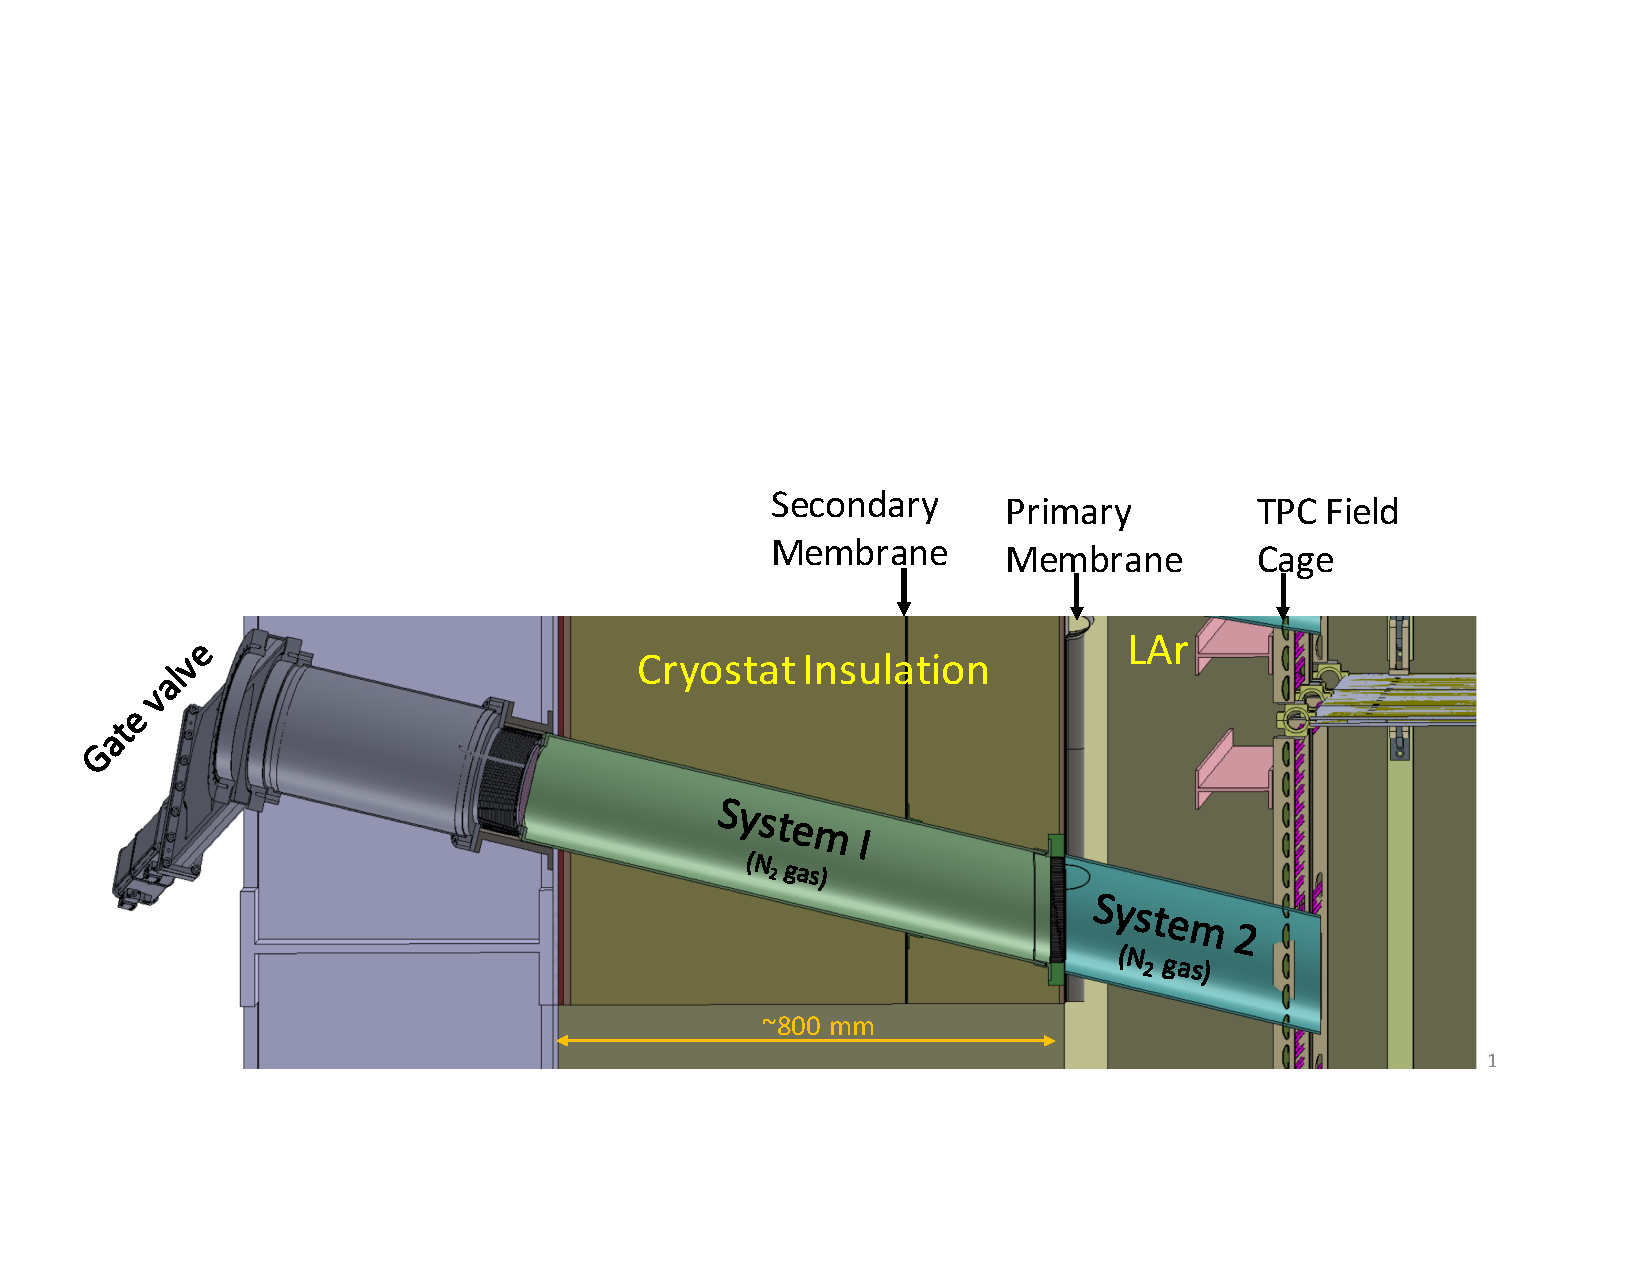
\includegraphics[width=0.90\textwidth]{beamwindow_system1and2.pdf}
%\end{cdrfigure}
%%%%%%%%%%%%%%%%%%%%%%%%%%%%
%Remove System 1 discussion
%%%%%%%%%%%%%%%%%%%%%%%%%%%
%\subsection{System 1}
%A close-up view of the System 1 beam window is shown in Figure~\ref{fig:beamwindow_zoom}. The system 1 beam window is a cylindrical G10 (OD$\approx$22cm) tube with a nomex honeycomb core at each end. The tube is filled with dry nitrogen gas and maintained at about 1 atm of pressure. It is designed to provide thermal insulation with a heat load of less than 5W/$m^2$. As shown in Figure~\ref{fig:beamwindow_fig1}, system 1 beam window extends to the external steel support structure of the cryostat. The other end of the beam window is in physical contact with the cryostat's primary membrane. When the cryostat is filled with LAr, the nomex honeycomb core provides the structural support to prevent the membrane from bulging outward. The honeycomb core on the other end of the tube, where the bellow is located, provides thermal insulation to keep ice from building up on the outer surface. The secondary membrane will be bonded onto a cylindrical disk attached to the G10 shell during installation. The system 1 beam window is anchored to the outer steel structure of the cryostat with a flange. As an additional safety measure, there is an option to install a gate valve on the external end of the beam window.
%\begin{cdrfigure}[Beam window 1 zoomed]{beamwindow_zoom}{A detailed view of system 1 beam widnow.}
%  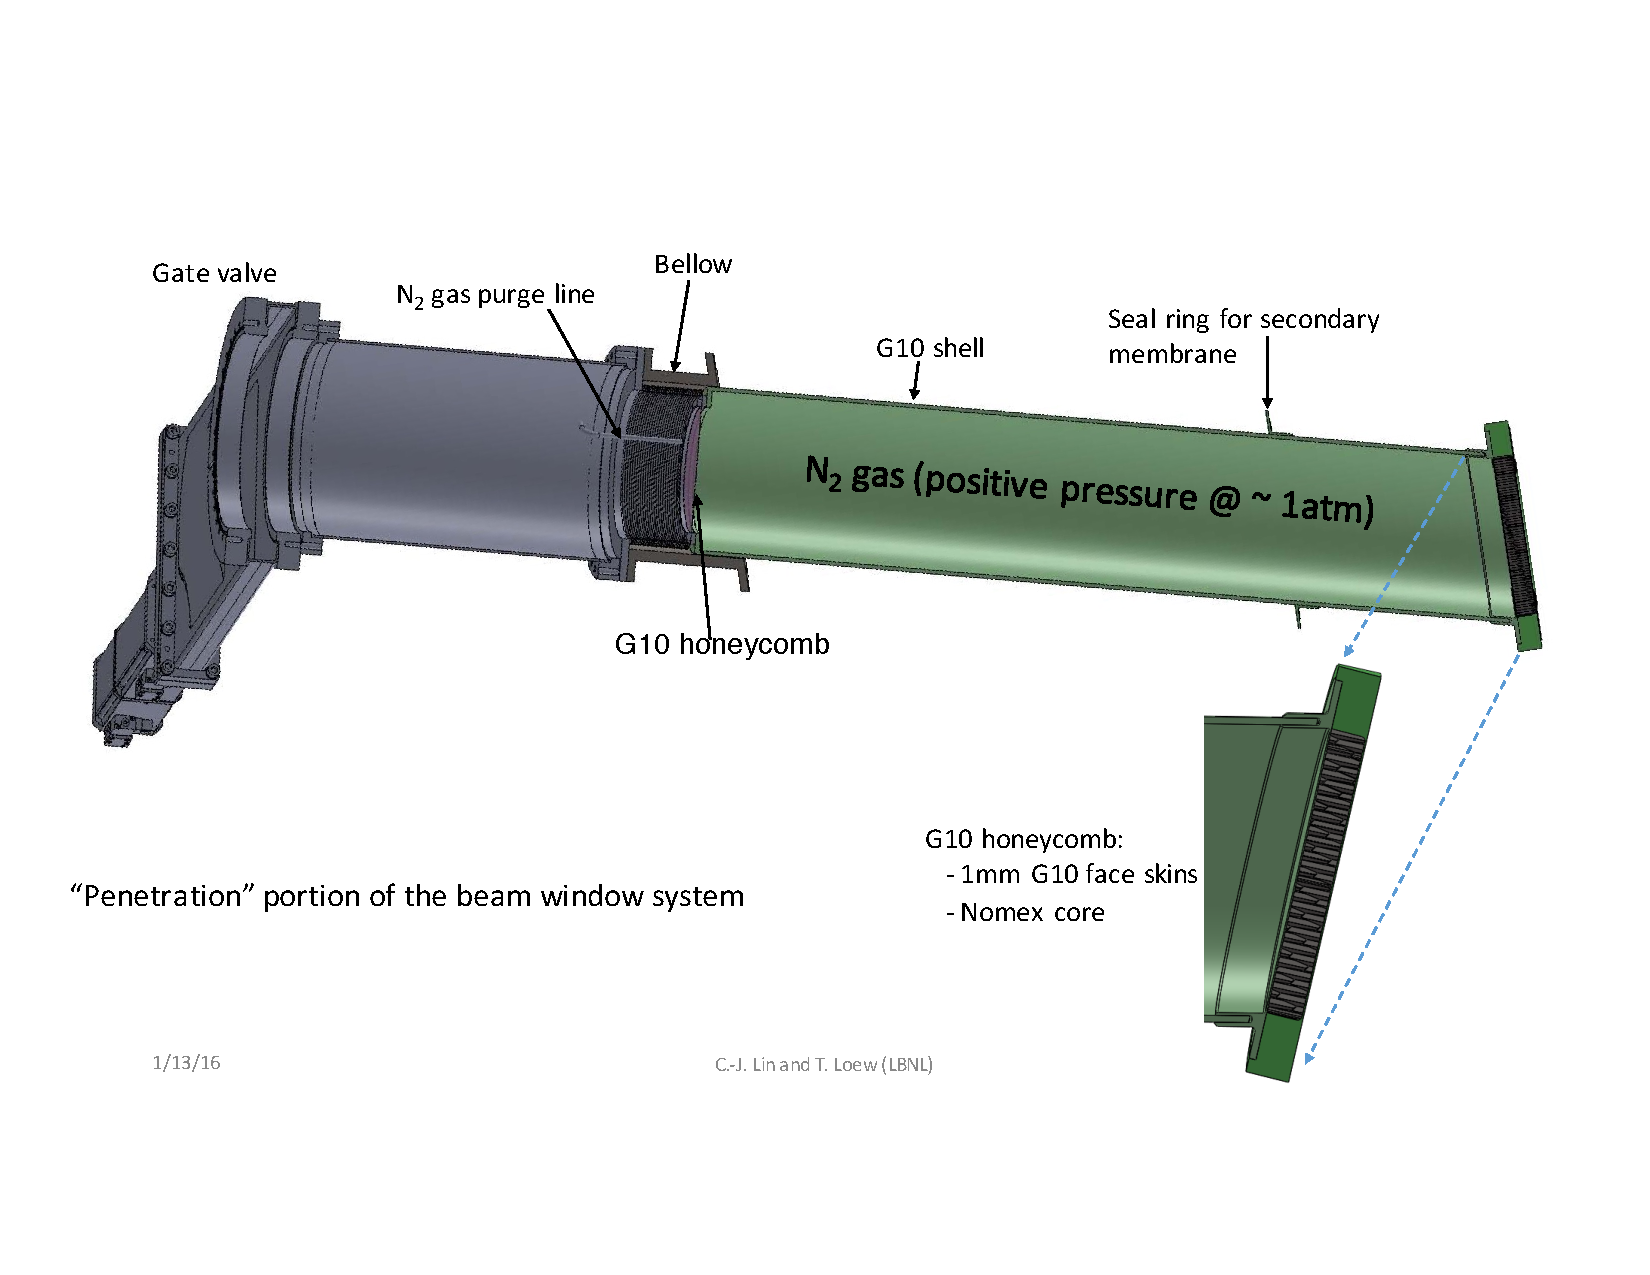
\includegraphics[width=0.90\textwidth]{beamwindow_system1zoom.pdf}
%\end{cdrfigure}

The beam plug is designed to displace the passive LAr layer between the TPC field cage and the inner cryostat membrane. As illustrated in Figure~\ref{fig:beamwindow_fig2}, it is a cylidrical glass-fiber composite pressure vessel about 50cm in length and  22cm in diameter. It is filled with dry nitrogen gas via a stainless steel line that extends to the top of the cryostat. The pressure inside the beam plug is maintained externally up to 25 psi from room to LAr temperatures. A pressure relief valve (or burst disk) will be installed on the nitrogen fill line on the top of the cryostat (externally) to ensure the pressure inside the beam plug does not exceed the safety level. The component-level view of the beam plug is shown in Figure~\ref{fig:beamplug_components}.  The beam plug is secured to the field cage support structure as described in Section~\ref{subsec:fc-beamplug}. The front portion of the beam plug extends about 5~cm inside the field cage through an opening in the field cage. The field cage support is designed with sufficient strength to withstand the weight of the beam plug while it is suspended in air. 
\fixme{what about a torque on the FC ?}
When the cryostat is filled with LAr, the beam plug is roughly neutrally buoyant.  The total internal volume of the beam plug is about 16 liters. 

The requirements on the acceptable leak rate is between $7.8\times 10^{-5}$ scc/s to $15.6\times 10^{-5}$ scc/s. This is a very conservative leak rate and is roughly equivalent to 15\% of the nitrogen in the vessel leaked over a period of a year.
\fixme{which nitrogen in the vessel ? Clarify whether these are material impurities or something else ? How do we know what the N is inside the cryostat ?}
  In a worst case scenario with all the nitrogen in the beam plug leaking into the LAr cryostat, the increase in concentration is about 0.1 ppm, which is still a factor of 10 below the acceptable level as specified by light detection requirements.
  \fixme{need some reference with details for this requirement}
  At nominal operation, the voltage difference across the beam plug could be as high as 165kV. 
  \fixme{add a one sentence explanation where "as high as 165kV" comes from - not constant at nominal operation ? }
  To minimize risk of electrical discharges, the beam plug is divided into sections and each section is bonded to stainless steel conductive grading rings. The grading rings are connected in series with two parallel path of resistor chains. There are 7 grading rings. The ring that is closest to the field cage is electrically connected to one of the field cage profiles. 
  The last ring near the cryostat wall is grounded to the stainless steel membrane. 
  \fixme{how is the connection to the membrane made without risking damage to the membrane ?}
  The type and value of the resistor is still under evaluation. A likely candidate is the high voltage Super Mox 15G$\Omega$ resistor by OHMITE. The maximum total power dissipated by the resistor chain is about 0.6W.


\begin{cdrfigure}[Beam plug]{beamwindow_fig2}{The beam plug is a  composite pressure vessel filled with dry nitrogen gas. The vessel is about 50cm in length and about 22cm in diameter. The pressure vessel is divided into sections with each section bonded to a stainless steel grading ring. The grading rings are connected by two parallel paths of resistor chain.}
  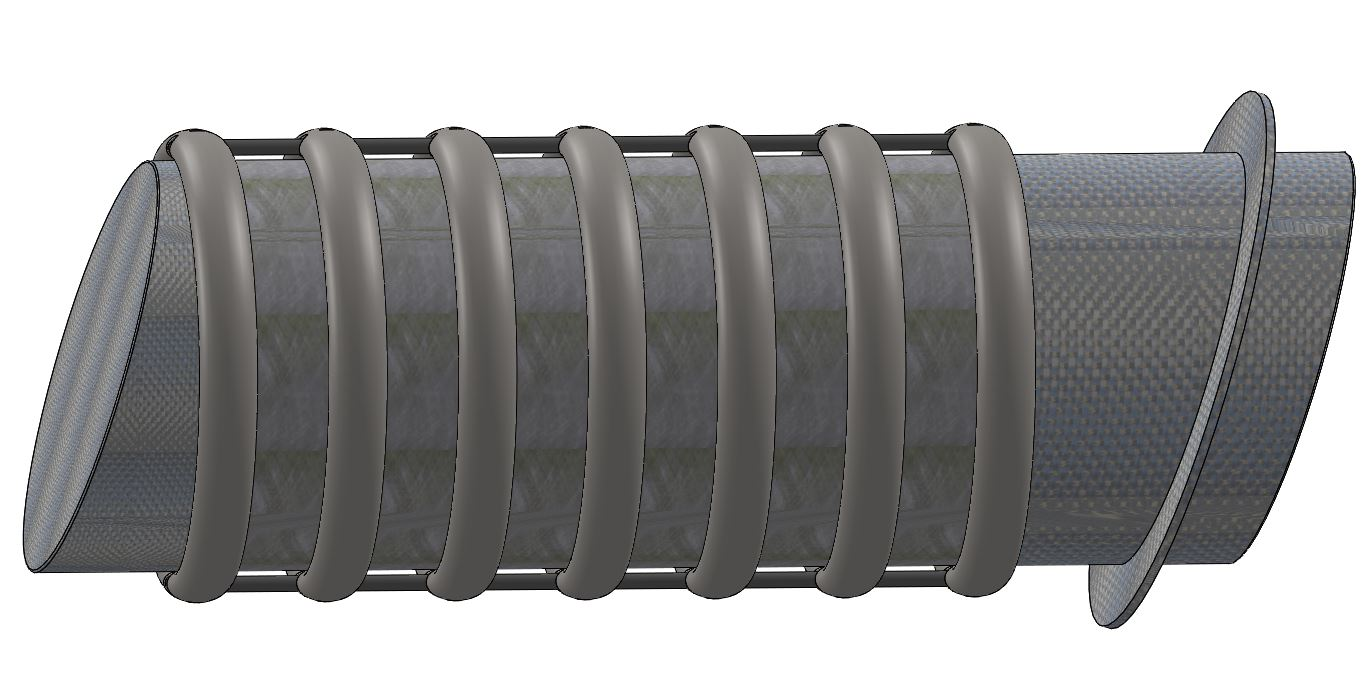
\includegraphics[width=0.5\textwidth]{beamwindow_system2.jpg}
\end{cdrfigure}

\begin{cdrfigure}[Beam plug component-level view]{beamplug_components}{Component-level view of the beam plug showing alternating electrode and composite ring structure.}
  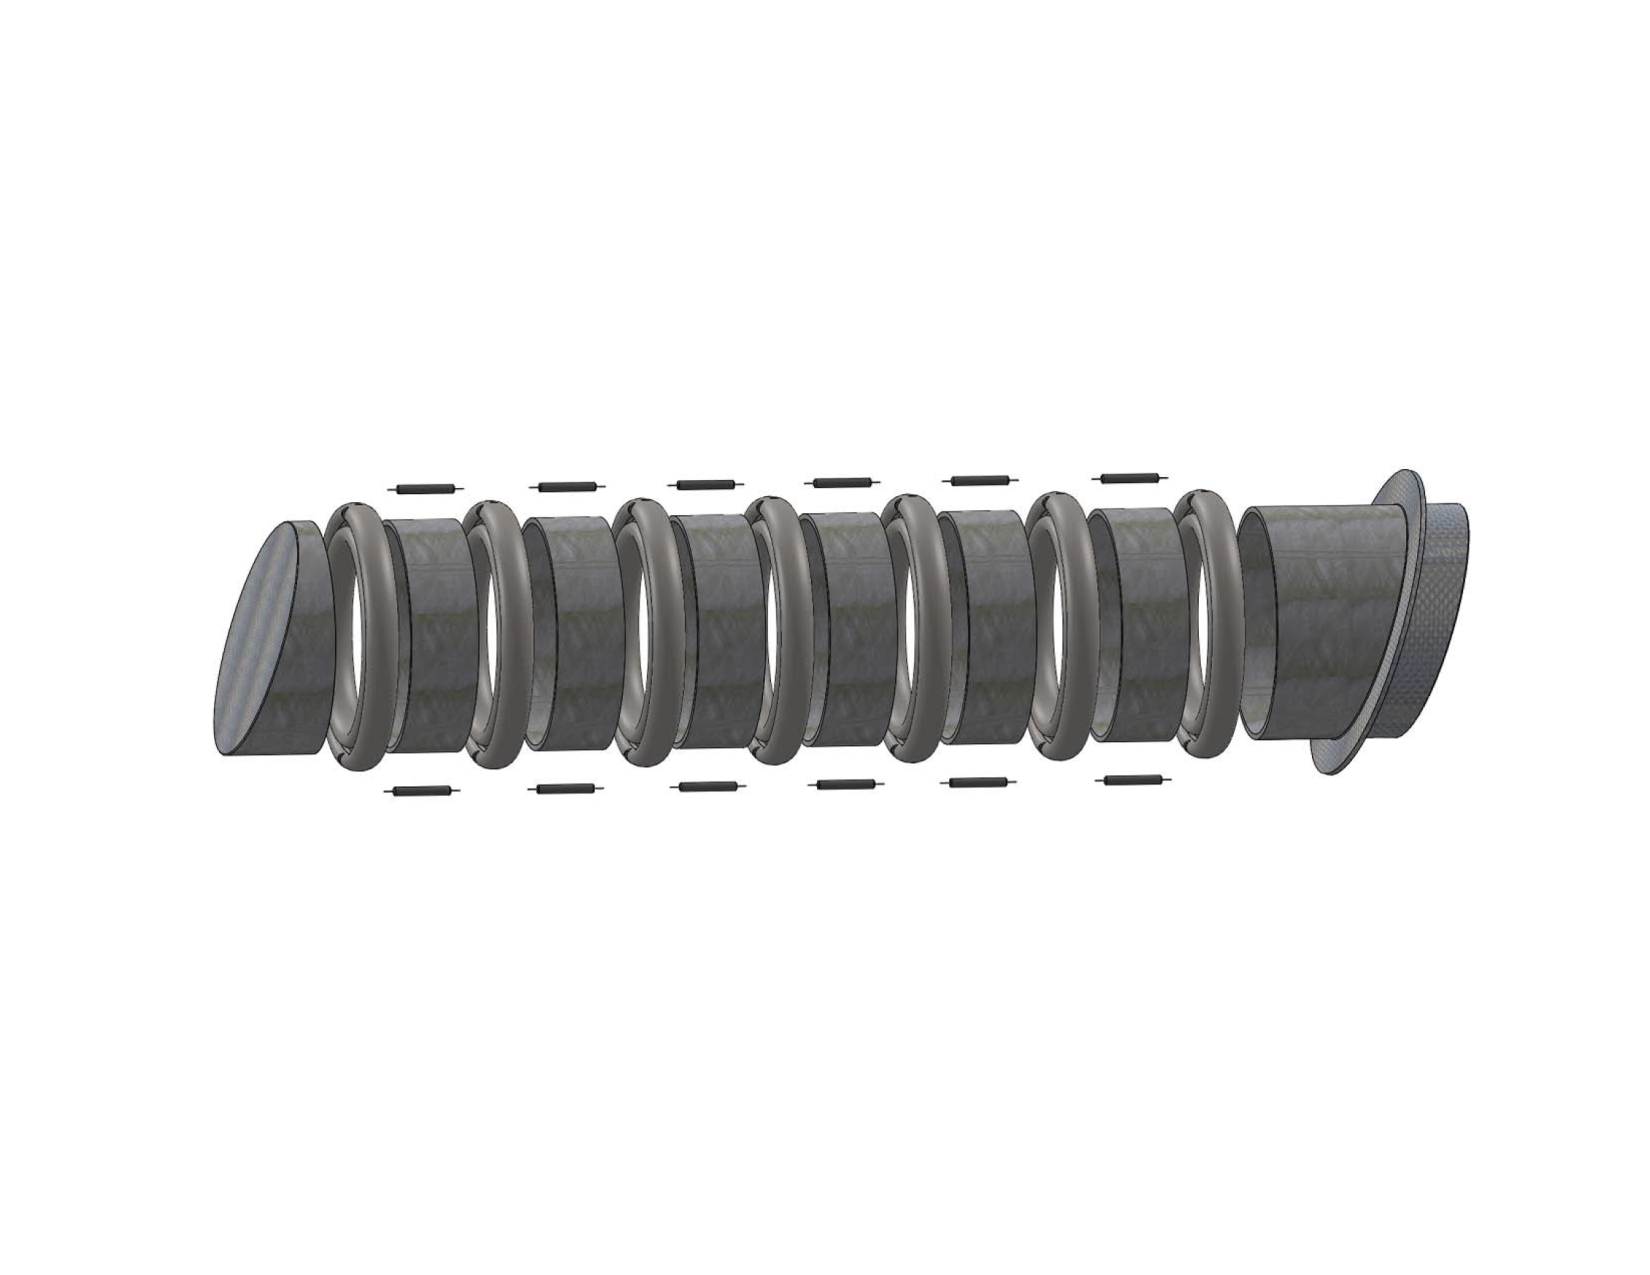
\includegraphics[width=0.85\textwidth]{beamplug_components.pdf}
\end{cdrfigure}

The metal electrode rings are spaced at regular intervals and interspersed with composite tube sections. The shape of the rings has been designed to minimize high electric field corners. The results of the field calculations are shown in Figures~\ref{fig:beamplug_ring1} and~\ref{fig:beamplug_ring2}. The average field in the vicinity of the beam plug is about 4.4 kV/cm. The maximum field of 15.7 kV/cm is on the electrode ring surface. In all regions the field is well below the 30 kV/cm limit.
\fixme{citation to doc describing limit would be good}

\begin{cdrfigure}[Beam plug electrodes]{beamplug_ring1}{Electric field calculation of the electrode ring design. The average field in the beam plug region is about 4.4 kV/cm. The maximum field of 15.7 kV/cm is on the electrode ring surface. }
  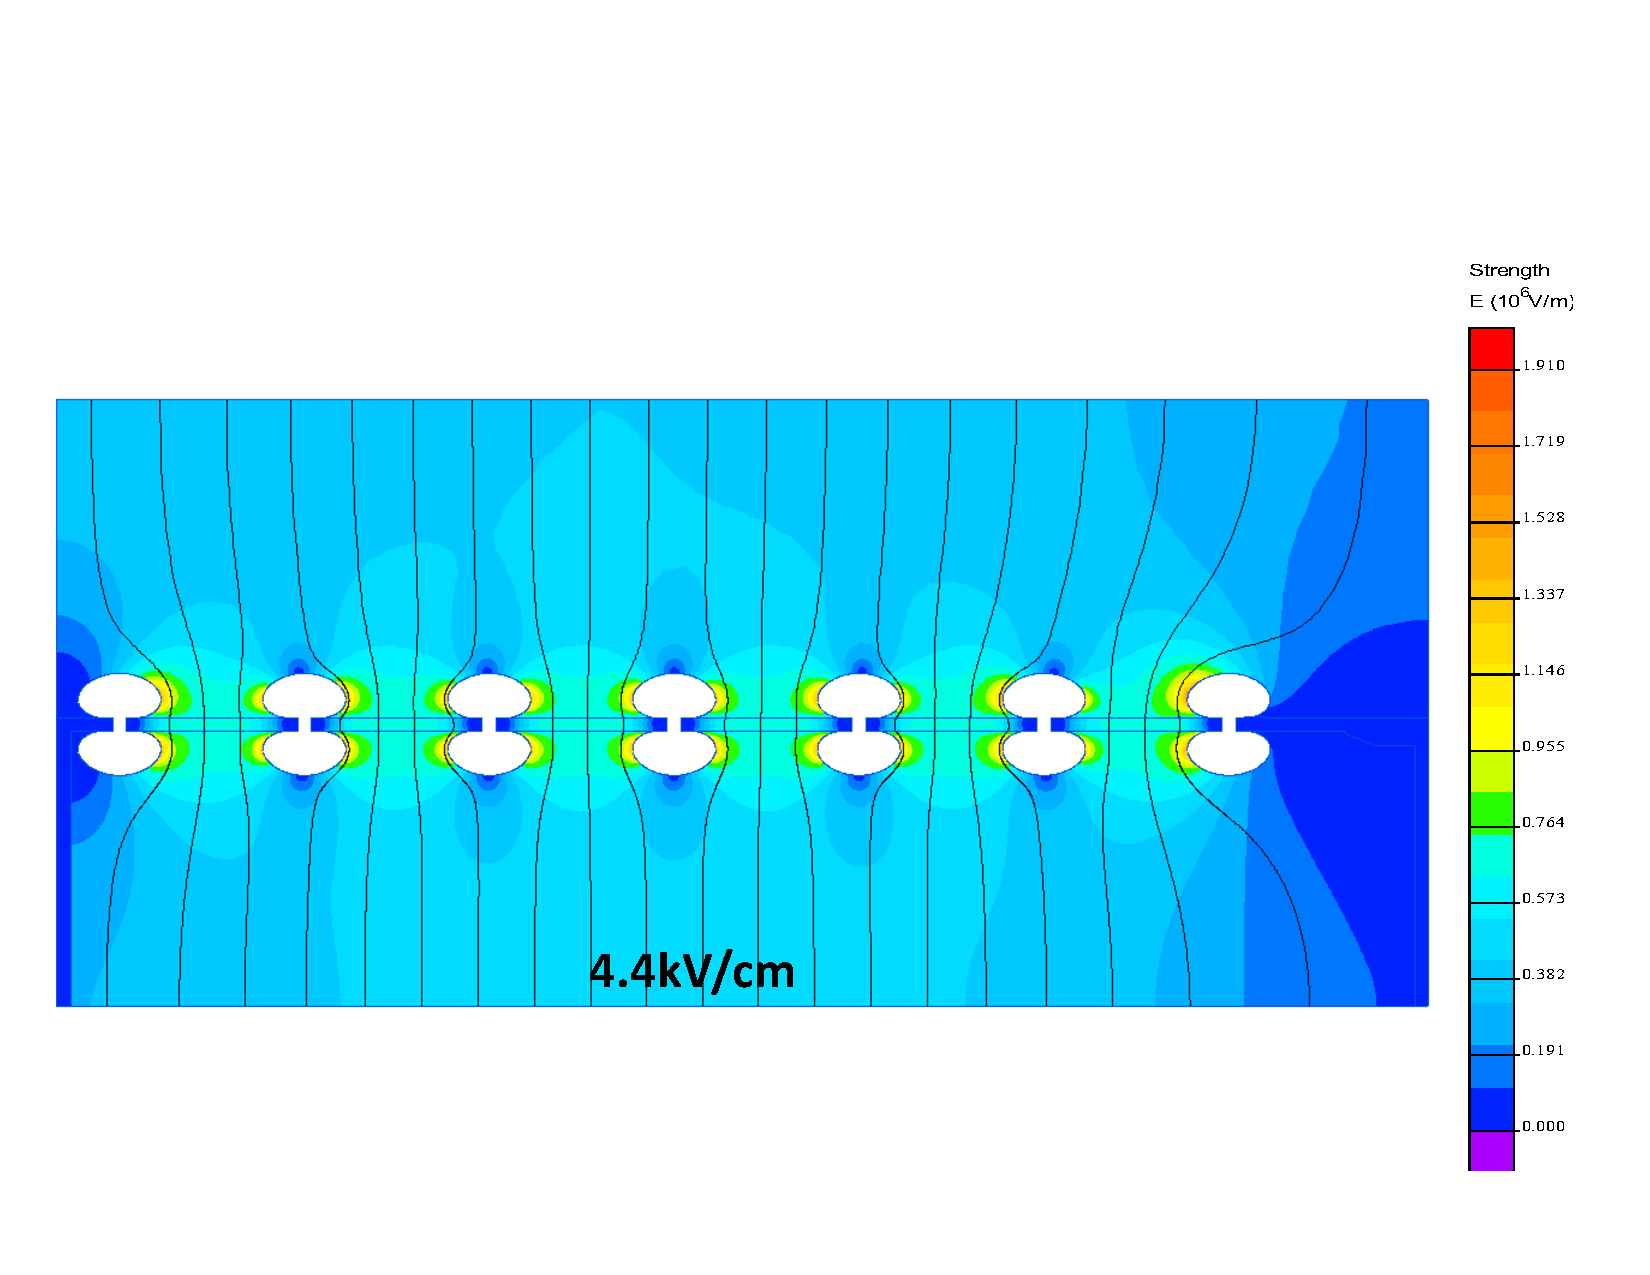
\includegraphics[width=0.85\textwidth]{beamplug_ring1.pdf}
\end{cdrfigure}

\begin{cdrfigure}[Beam plug electrode]{beamplug_ring2}{Electric field calculation near the vicinity of the electrode. The shape of the ring minimizes the high field region near the joints between the electrode, LAr, and composite shell. The field is well below the 30 kV/cm limit in all regions.}
  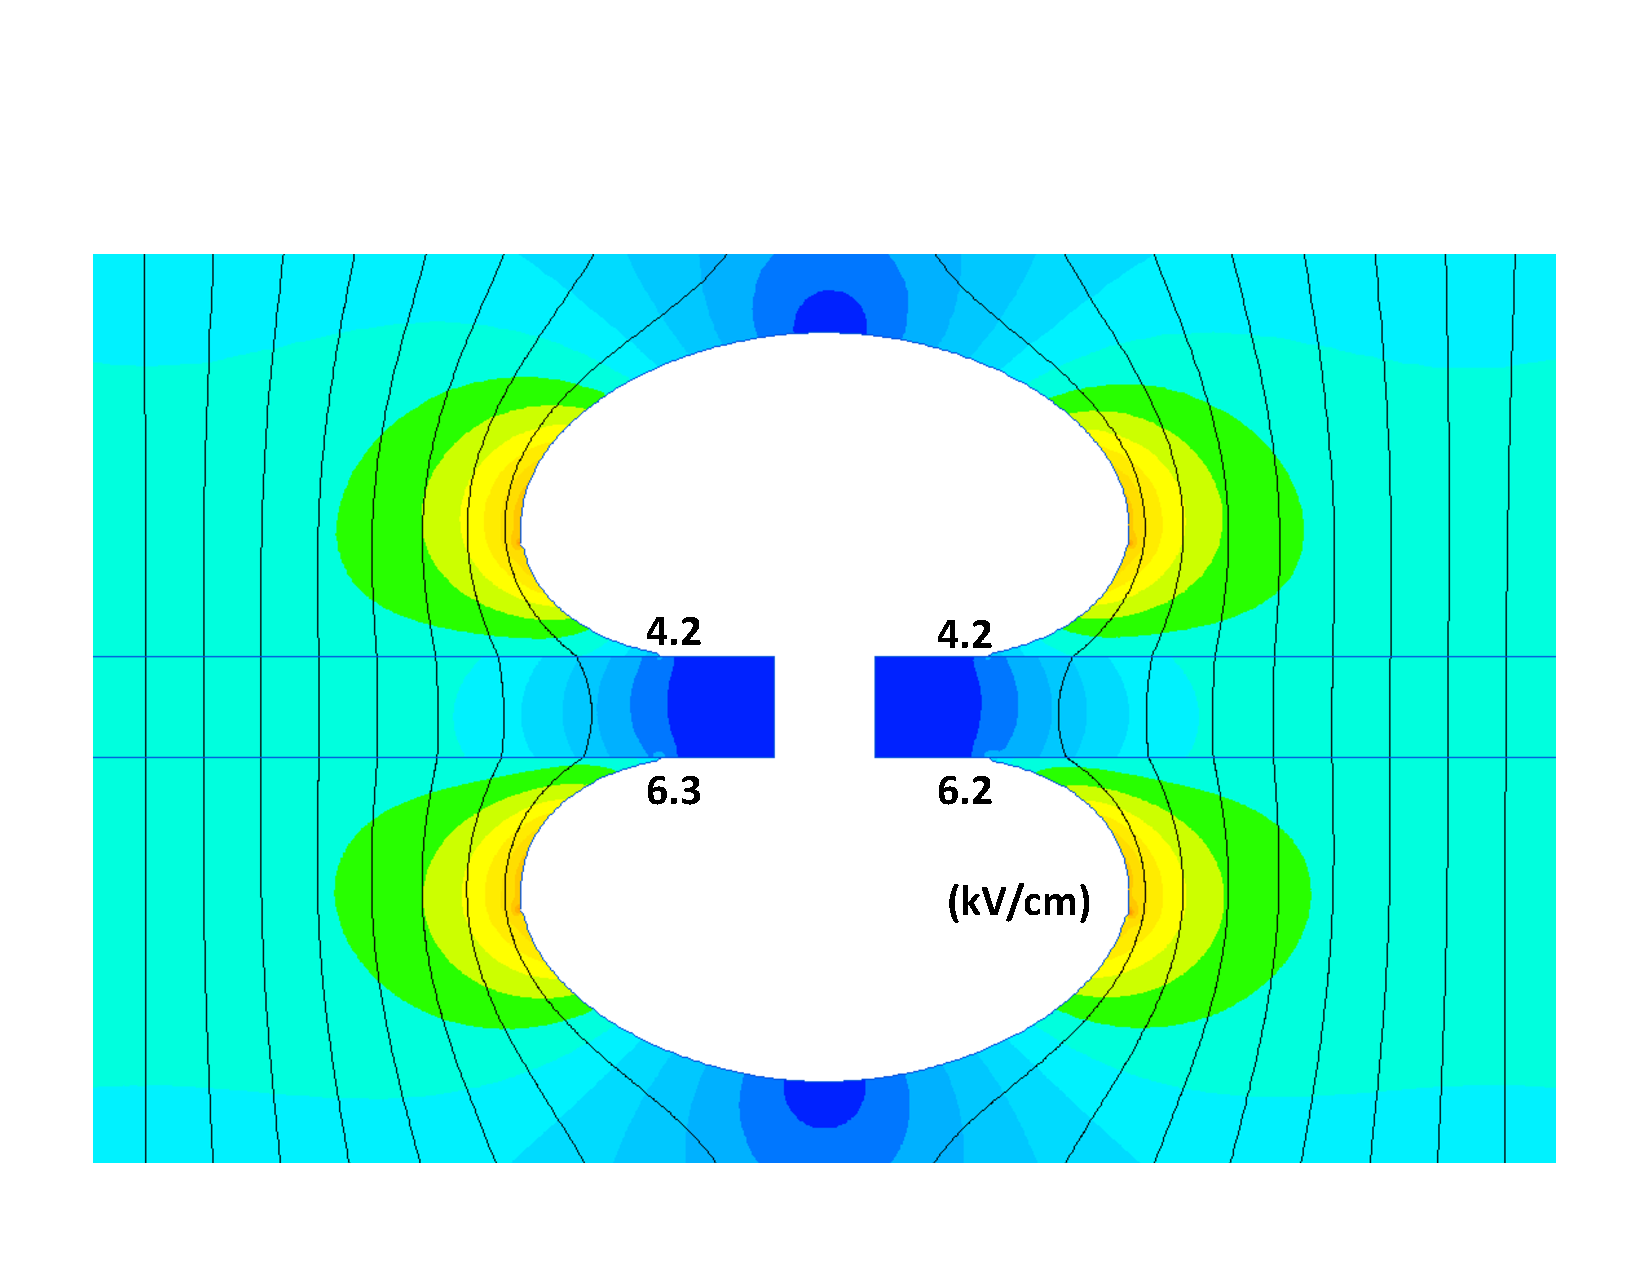
\includegraphics[width=0.5\textwidth]{beamplug_ring2.pdf}
\end{cdrfigure}

A summary of the beam plug requirements and parameters list are given in Table~\ref{tab:bprequirements}.

\begin{cdrtable}[Beam plug requirements]{lll}{bprequirements}{Beam plug requirements and parameters list}
Parameter & Value & Notes \\ \toprowrule
Dimensions & & Defined by CAD model \\ 
~~Internal Diameter (est) & 200~mm & At composite ring ID surface; \\
                          &        & tolerance for assembly \\ 
~~Wall thickness (est) & 8~mm & Tolerance for assembly \\ 
~~Length (est) & 495~mm $\pm$ 1~mm & Overall (Normal Distance) \\ 
               & 577~mm $\pm$ 1~mm & Overall (Absolute Distance) \\ \colhline 
Metal End Cap Angle & (16.2$\pm$0.25)$^\circ$ & From perpendicular; \\ 
                    &                         &maintain length tolerance \\ 
Composite End Cap   & (16.2$\pm$0.5)$^\circ$ & From perpendicular; \\ 
                    &                        & maintain length tolerance \\ 
Flange Angle        & (16.2$\pm$0.25)$^\circ$ & From perpendicular \\ \colhline 
Tolerances  & ASME Y14.5 2009 & Where useful to convey design intent \\
            &                 & and function \\ 
Materials used   & & Electrically insulating; selected from or\\
                 & & approved per FNAL LAr purity list \\ 
Epoxy system & Hysol 9309.2 NA & Rated for cryogenic use\\
Electrode Rings & 304 Stainless steel & \\ \colhline 
Resistor Type & OHMITE Super-Mox 930 Series & \\
Resistor Value & 15~G$\Omega$ & \\
Number of resistors & 6 & \\
Power dissipation &  &\\ 
~~Per resistor    & $\approx$0.1W & \\
~~Total           & $\approx$0.6W & \\ \colhline 
Operating Voltage & Up to 180 kV end-to-end & Electrically insulative \\ 
Operating Temperature & 25$^\circ$~C & Room temperature \\ 
                      & -185$^\circ$~C & LAr temperature \\ 
Operating Pressure    & 25~psi & MAWP at operating temperature \\ \colhline
Pressure Environment & 14.7 psi & Ambient temperature \\
(External)           & 19.9 psi & LAr temperature \\ \colhline
Internal Volume & 15.5 liter (est.) & Internal \\
                & 22 liter (est.) & External displacement \\ \colhline
Permeability/Leak Rate  & 7.8$\times$10$^{-5}$ scc/s to & He gas equivalent \\
Range                             & 15.6$\times$10$^{-5}$ scc/s \\ \colhline
Operating Lifetime   & 1 yr  &  \\
Lifetime Operational Thermal & 4 & \\
~Cycles to 77 K & & \\ \colhline
Shock Loading & & No design shock loading \\
Vibration Loading & & No design vibration loading \\ \colhline
Flange Profile & & Geometry per LBNL ICD \\
Weight (est.) & 75 lb [34 kg] & With SS304 electrode rings \\
Buoyancy Load (est.) & 67.5 lb [31 kg] & \\
Pressure Port & & Ground cap interface per LBNL \\ \colhline
Design Safety Factor & 2 & On MAWP (=50 psi) \\
Pressure Test Factor & 1.5 & Pneumatic test \\
High Voltage Tests & (180 kV equivalent) & \\ 
\end{cdrtable}



\subsection{Field cage resistor divider chain with beam plug}
The resistor divider chain of the beam plug is tied to the main field cage profile. To maintain the 3 kV voltage drop across all field cage profiles, a second resistor divider board is added in parallel to the nominal board for the first 5 field cage profiles closest to the CPA. This modification is only needed for the field cage panel with the beam plug attached. The circuit diagram for the proposed scheme and the resistor values are shown in Figure~\ref{fig:beamplug_resistordivider}.
\begin{cdrfigure}[Beam plug resistor divider chain]{beamplug_resistordivider}{The resistor divider circuit for the end-wall field cage panel with the beam plug. The proposed resistor values for the main, parallel divider boards, and the beam plug are given in the tables.}
  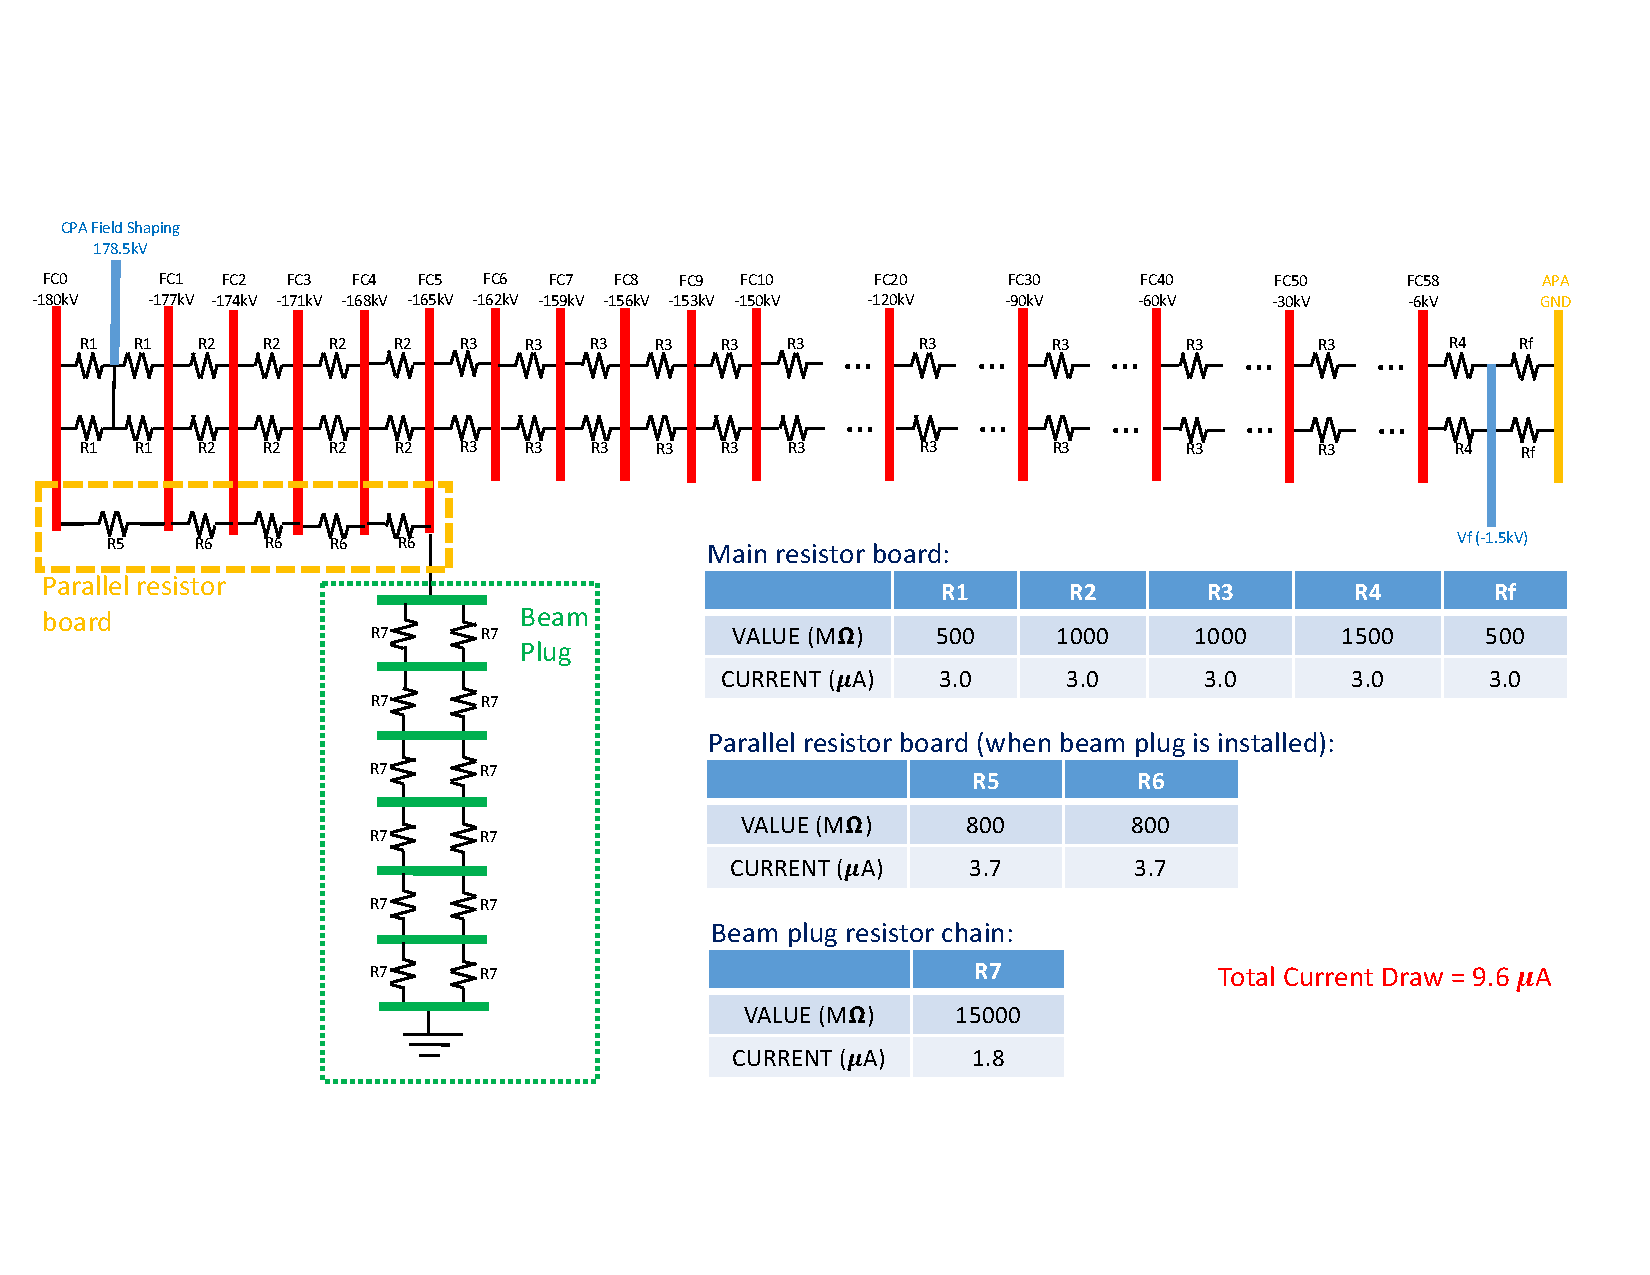
\includegraphics[width=0.85\textwidth]{beamplug_resistordivider.pdf}
\end{cdrfigure}
\fixme{why is there a labeling of R2 and R3 as well as R5 and R6 when these are the same ?? please simplify}

\subsection{Component performance tests}

\paragraph{Adhesive shear testing of ring joints}
The stainless steel electrodes and the composite shells will be bonded using a cryogenically rated epoxy system (Hysol 9309.2 NA). Prototype components that match the beam plug geometry have been fabricated and used to measure the adhesive shear strength for the proposed joints. The measurements were done at cryogenic temperature and also as a function of bond length and component shell thickness. 
\fixme{shear strength was really measured in LN ?? How ? }
Testing results indicate that the default design has at least a safety factor of 6 for axial adhesive shear failure. The test samples and setup are shown in Figure~\ref{fig:beamplug_sheartest}.

\begin{cdrfigure}[Beam plug Shear Test]{beamplug_sheartest}{Photo on the left shows the bonded test samples. The measurements were performed for different bond lengths and composite shell thicknesses. Photo on the right shows the test setup. The tests were done at LN temperature.}
  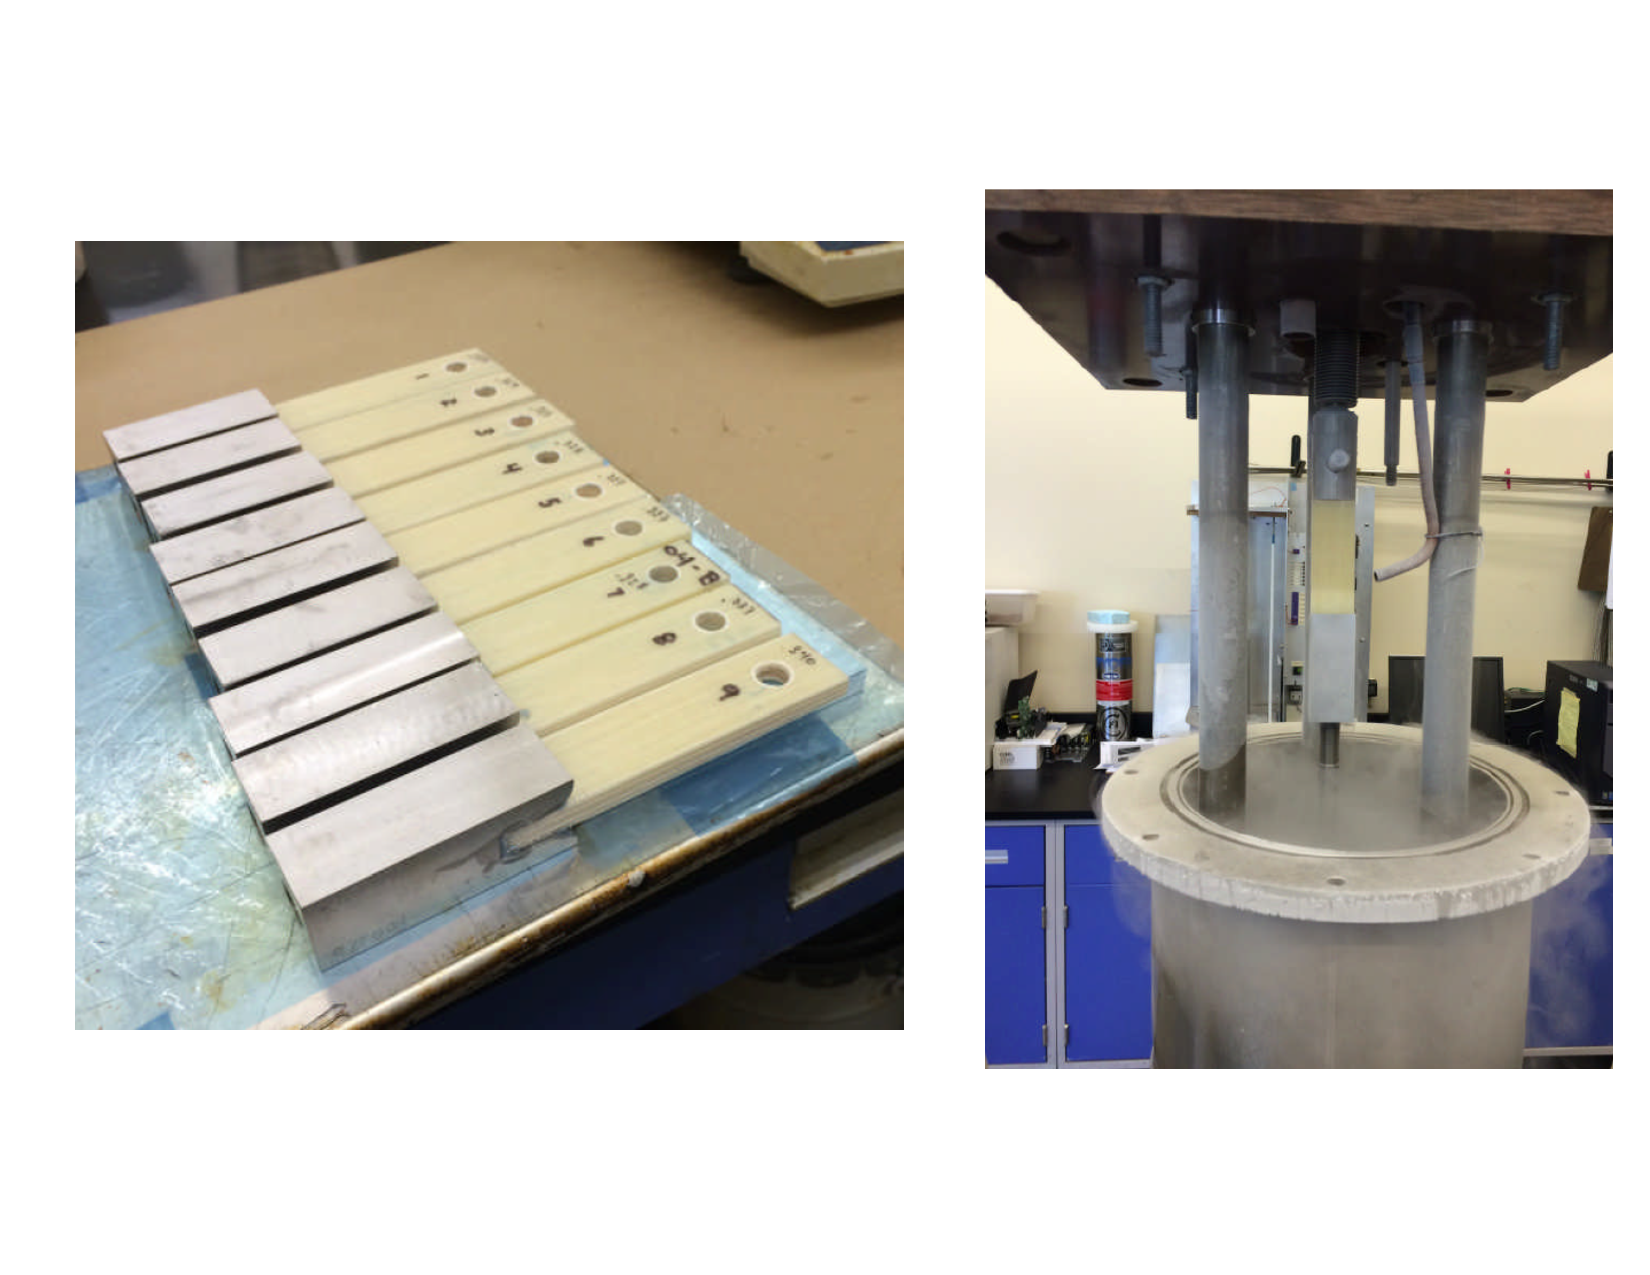
\includegraphics[width=0.75\textwidth]{beamplug_sheartest.pdf}
\end{cdrfigure}
\fixme{could remove right panel of figure - or add better labeling}

\paragraph{Dielectric strength of composite shell}
The pressure vessel material is composed of electrically insulative glass fiber composite. Samples of the materials were obtained from the vendor and tested at LBNL for dielectric breakdown along the composite surface. The test setup is shown in Figure~\ref{fig:beamplug_dielectric}. The test samples and electrodes were fabricated to match the beam plug geometry. The material samples were successfully tested at room temperature in air up to about 50 kV, which is the limit of the test in air. This is about a factor of two higher than our nominal voltage between electrodes.
\fixme{Add sentence to say what exactly was tested: physical damage due to HV, or ... ?}
\begin{cdrfigure}[Dielectric strength test]{beamplug_dielectric}{Test setup to measure the dielectric breakdown of the composite material. The sample tested is shown in the photo on the left. The composite plate is attached to the electrodes that have been machined to match the geometry of the beam plug. The photo on the right shows the HV connection.}
  \includegraphics[width=0.85\textwidth]{beamplug_dielectric.pdf}
\end{cdrfigure}


%\begin{cdrfigure}[System 2 beam window mounting scheme]{beamwindow_fig3}{System 2 beam window mounting scheme (preliminary). The beam plug is mounted to the field cage support structure.}
%  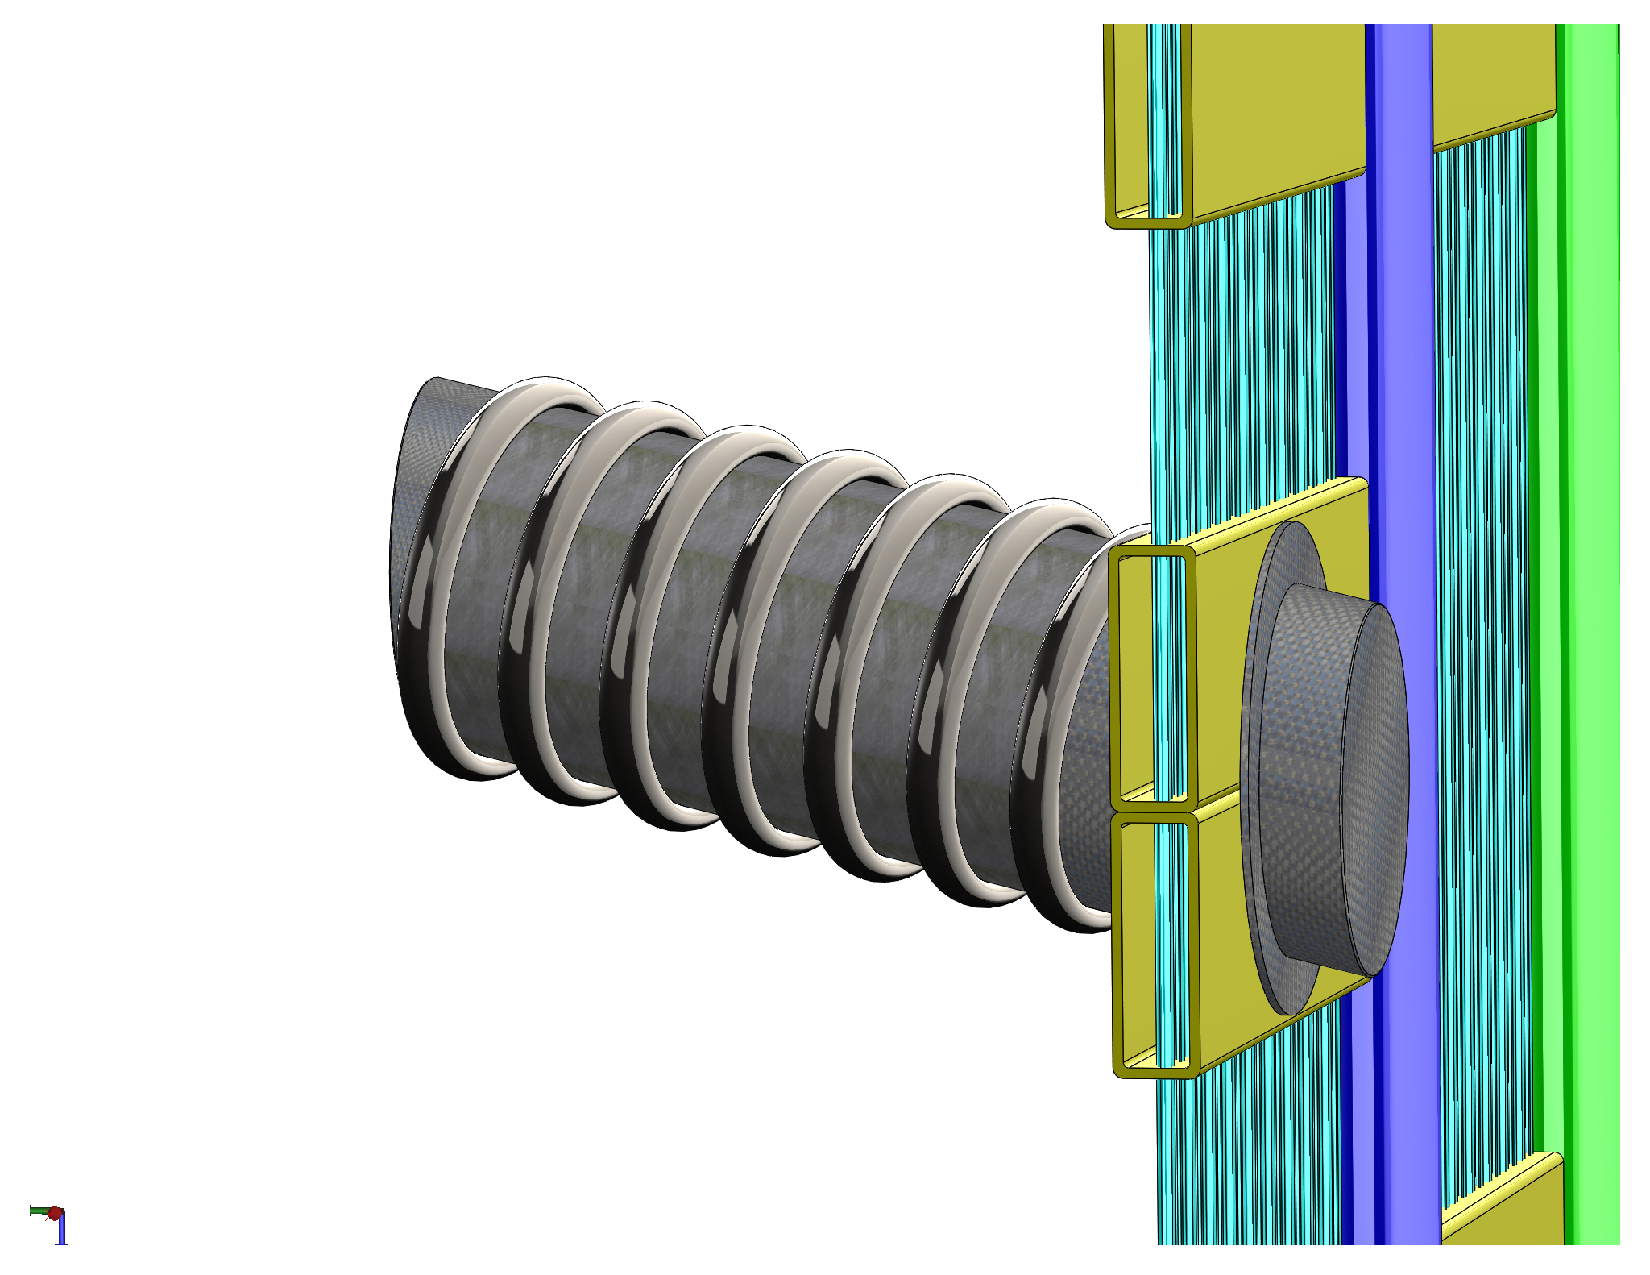
\includegraphics[width=0.7\textwidth,height=0.3\textheight]{beamwindow_system2_mount.pdf}
%\end{cdrfigure}



%%%%%%%%%%%%%%%%%%%%%%%%%
\subsection{QC Procedures}

As a part of the QC process for the beam plug, the vendor will conduct the following acceptance tests for the production units before shipping:
\begin{itemize}
\item {Initial helium leak check}
\item {Internal pressure check at cryogenic temperature (at about 2x operating pressure)}
\item {Post-test helium leak check to assess potential damage}
\item {External pressure check at room temperature (below 100 psi)}
\item {Final helium leak check to ensure no damage has been incurred}
\end{itemize}
\fixme{specify to what leak level test will be performed}
The acceptance tests performed by the vendor are primarily related to pressure safety and leak rates. Some of those tests will be repeated by LBNL upon receiving the units to verify vendor's results. In addition, LBNL will conduct tests to verify other aspects of the beam plug, in particular, the HV characteristics. The HV tests will be conducted using various facilities as described in the following sections.

\paragraph{BLANCHE Test Stand}
The BLANCHE test stand at Fermilab is a LAr cryostat dedicated to study high voltage related issues. It is 152 cm tall with a 76 cm inner diameter. The test stand is connected to a LAr purification system to remove oxygen and water contamination. The test stand is capable of delivering up to 150 kV to the sample. The cryostat is large enough to test a full size beam plug. The plan is to test the beam plug in BLANCHE to verify that the beam plug can withstand HV in LAr environment.
\\fixme{earlier nominal value across beam plug was said to be 165kV - so, test is not covering full range. Maybe add sentence to address this issue.}

\paragraph{Test in Charged Particle Beam}
During ProtoDUNE-SP physics runs, a charged particle beam will go through the beam plug with a rate of up to 100 Hz during a beam spill. The current induced from the ionization of the nitrogen gas by the charged beam particles is expected to be small; less than 1 nA during the spill. Given the low ionization rate and long pause between spills, we do not expect the charged particle beam to introduce electrical breakdown inside the beam plug. However, we plan to verify the design by putting the beam plug in a test beam with the beam plug at nominal HV. We will study the current flow inside the beam plug as a function of beam rate and nitrogen gas pressure. To minimize possible HV breakdown on the outer surface of the beam plug, which may complicate the interpretation of the test results, the beam plug will be immersed in dielectric oil. The test apparatus with the beam plug installed inside the setup is shown in Figure~\ref{fig:beamwindow_SLAC}.
\begin{cdrfigure}[SLAC beam test]{beamwindow_SLAC}{Beamplug test setup in electron beam to test electrical breakdown in the N filler gas.}
  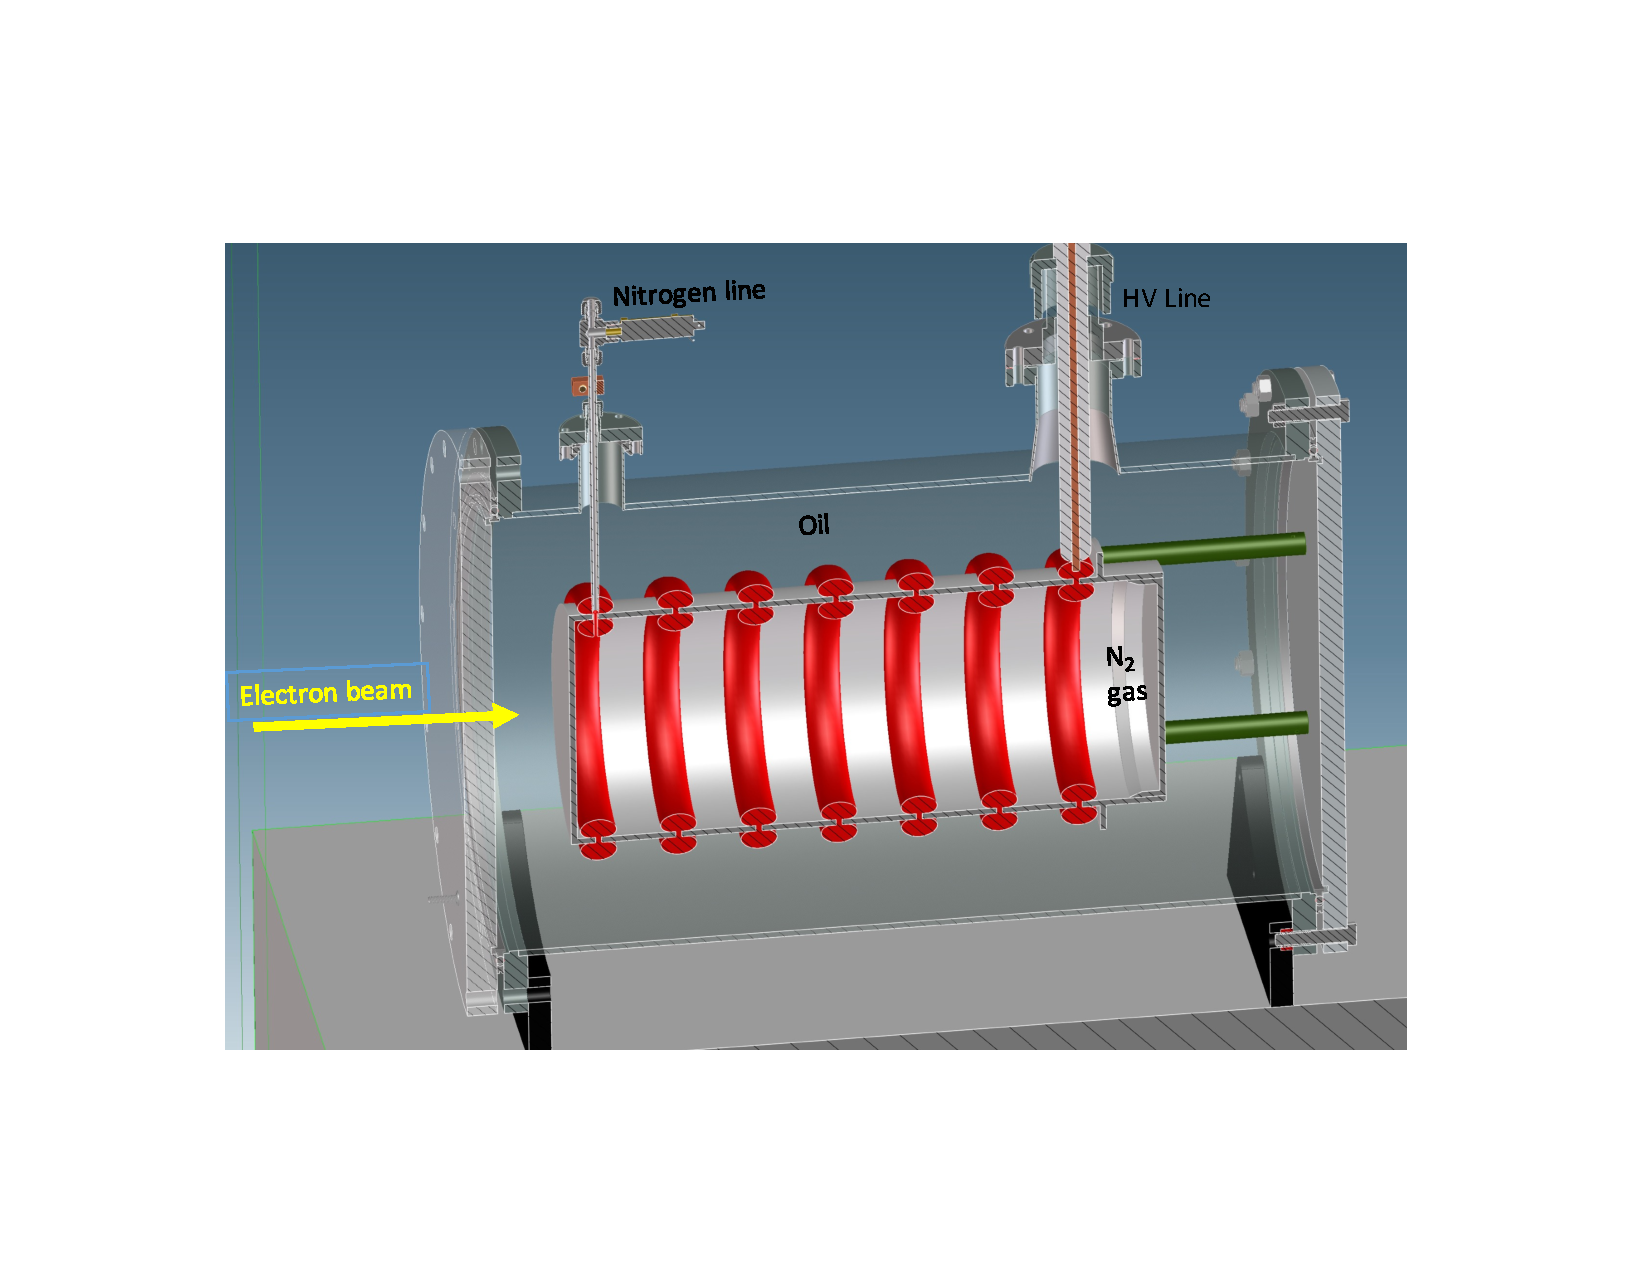
\includegraphics[width=0.6\textwidth]{beamwindow_SLACtest.pdf}
\end{cdrfigure}

\paragraph{Full integration test in 35-ton cryostat}
The final QC test of the beam plug is conducted inside the 35-ton cryostat at Fermilab. A small field cage mock-up is constructed and assembled inside the cryostat along with the beam plug. For this test, the beam plug is mounted to the field cage using a mounting scheme which is identical to the ProtoDUNE-SP one. The field cage mock-up will only have the first 10 profiles of a TPC, however, they will be operating at the nominal voltages. Therefore, the planned test will be a full-field test with the beam plug integrated into the field cage and the rest of the HV systems. A successful test would entail operating the TPC at the nominal HV (CPA at -180 kV) with the beam plug attached and that the electrical performance of the field cage with and without the beam plug is functionally the same.

\begin{cdrfigure}[PC4 Test setup]{beamwindow_PC4}{Field cage mock-up high voltage test in 35-ton cryostat \fixme{preliminary drawing}.}
  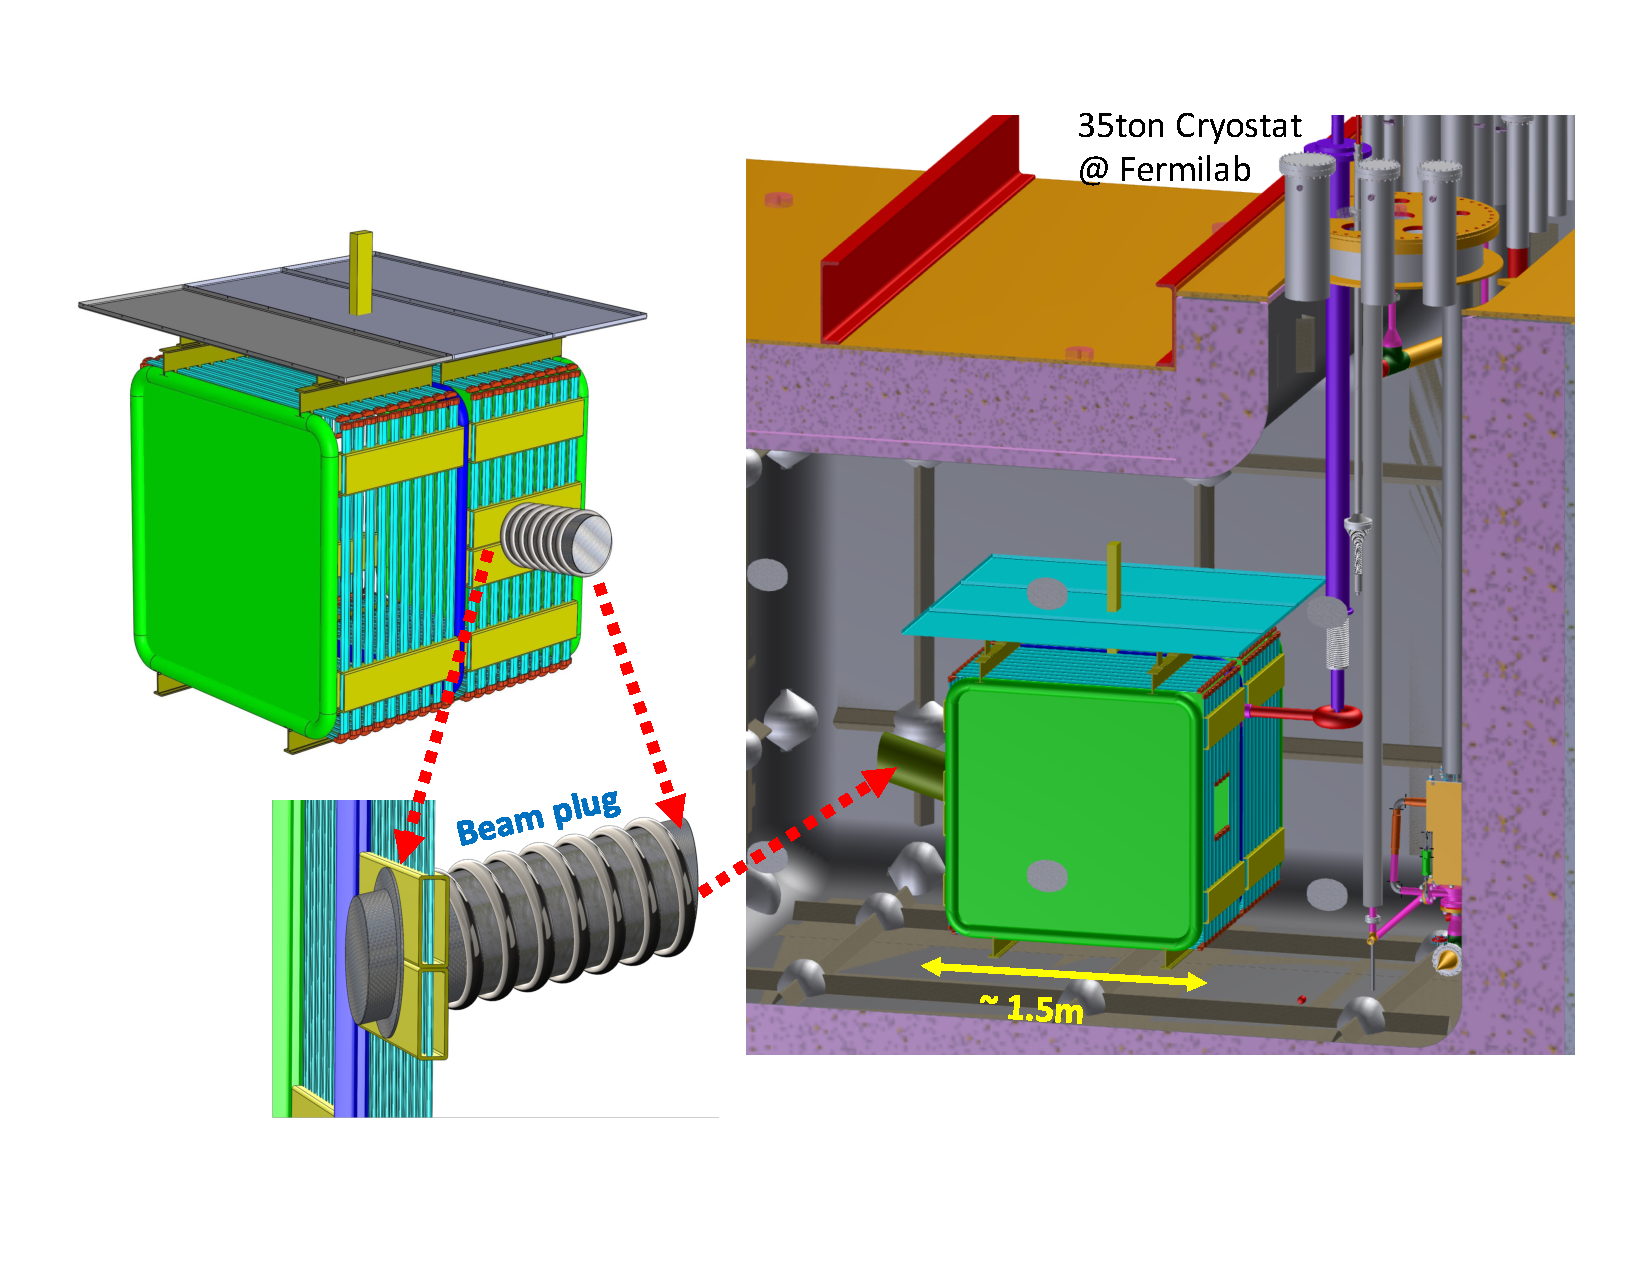
\includegraphics[width=0.95\textwidth]{beamwindow_PC4Test.pdf}
\end{cdrfigure}


